%% Template.tex; Solar Physics
%% 
\documentclass[namedreferences]{SolarPhysics}
%
% spr-sola-addons available options:
%  natbib        -- For citations: redefine \cite commands
%  solaenum      -- makes enumerated list with italics-roman numerals and a single right-bracket
%  linksfromyear -- loads a natbib and puts a link on a year citation (hyperref must be loaded)
%  optionalrh    -- for optional running title/author
%
\usepackage[optionalrh,solaenum]{spr-sola-addons} % For Solar Physics 
%\usepackage{epsfig}                     % For eps figures, old commands
\usepackage{graphicx}                    % For eps figures, newer & more powerfull
%\usepackage{courier}                    % Change the \texttt command to courier style
%\usepackage{amssymb}                    % useful mathematical symbols
\usepackage{color}                       % For color text: \color command
\usepackage{url}                         % For breaking URLs easily trough lines
\def\UrlFont{\sf}                        % define the fonts for the URLs


%% Local definitions
%% please place your own definitions here and don't use \def but
%% \newcommand{}{} or 
%% \renewcommand{}{} if it is already defined in LaTeX



%%%%%%%%%%%%%%%%%%%%%%%%%%%%%%%%%%%%%%%%%%%%%%%%%%%%%%%%%%%%%%%%%%
\begin{document}

\begin{article}

\begin{opening}

\title{THE HELIO 100 CME CHALLENGE}

%%%%%%%%%%%%%%%%%%%%%%%%%%%%%%%%%%%%%%%%%%%%%%%%%%%
%% Authors Names
%
\author{I.~\surname{}%$^{1}$\sep
%        I.~\surname{}$^{1}$\sep
%        I.~\surname{}$^{2}$      
       }

%%%%%%%%%%%%%%%%%%%%%%%%%%%%%%%%%%%%%%%%%%%%%%%%%%%
%% Runningheads
%
%\runningauthor{}
%\runningtitle{}


%%%%%%%%%%%%%%%%%%%%%%%%%%%%%%%%%%%%%%%%%%%%%%%%%%%
%% Affilations 
%
  \institute{$^{1}$ First affiliation
                     email: \url{e.mail-a} email: \url{e.mail-b}%\\ 
%             $^{2}$ Second affiliation
%                     email: \url{e.mail-c} \\
             }


%%%%%%%%%%%%%%%%%%%%%%%%%%%%%%%%%%%%%%%%%%%%%%%%%%%
%%% Abstract 
\begin{abstract}

This Challenge will focus on using HELIO to study the origin, propagation and impacts of a large number of Coronal Mass Ejections (CMEs) in the Heliosphere. HELIO provides an interface that allows researchers to track active regions as they evolve and produce solar flares and CMEs. Once launched, CMEs can be tracked in coronagraph and heliospheric images. Their impacts throughout the Heliosphere can then be measured using in-situ instruments from a number of spacecraft throughout the Heliosphere. The aim of this Challenge is to use HELIO to track a large number of CMEs (e.g., 100) from the surface of the Sun to their effects through interplanetary space and at the planets.

\end{abstract}



%%%%%%%%%%%%%%%%%%%%%%%%%%%%%%%%%%%%%%%%%%%%%%%%%%%
%% Keywords
%
%\keywords{}


\end{opening}
%-------------------------------------------------

%%%%%%%%%%%%%%%%%%%%%%%%%%%%%%%%%%%%%%%%%%%%%%%%%%%
%% Sections
%
% \section{}%\label{s:?} 
\section{Introduction}

\begin{figure} 
\centerline{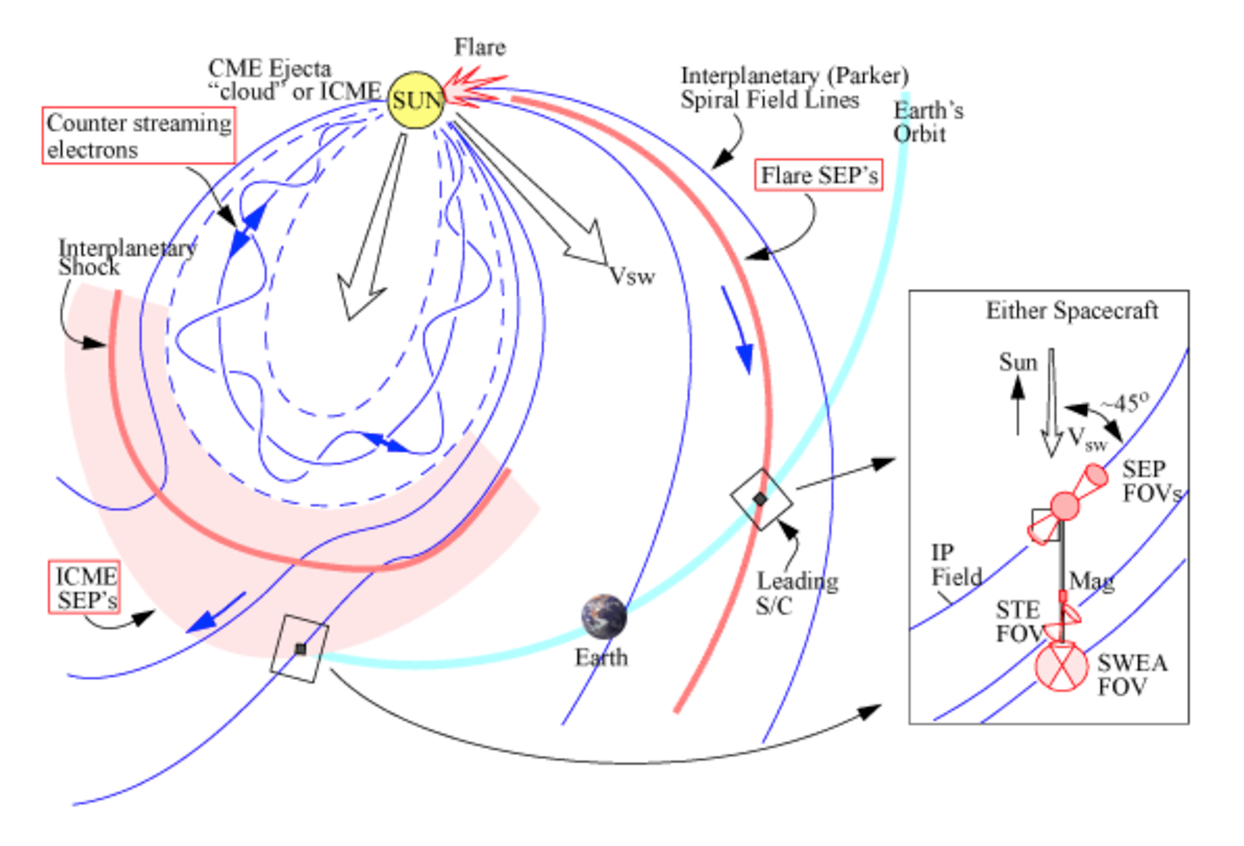
\includegraphics[width=0.5\textwidth,clip=]{images/science_of_impact_c.pdf}}
\caption{}%\label{fig:?}
\end{figure}

\section{Building a workflow}

The HELIO




%% Figure 
%
% \begin{figure} 
% \centerline{\includegraphics[width=0.5\textwidth,clip=]{<fig.eps>}}
% \caption{}%\label{fig:?}
% \end{figure}



%% Table
%
% \begin{table}
% \caption{}%\label{tbl:?}
% \begin{tabular}{}     
% \hline
% \multicolumn{2}{c}{<>}
% <data>
% \hline
% \end{tabular}
% \end{table}
  

%%%%%%%%%%%%%%%%%%%%%%%%%%%%%%%%%%%%%%%%%%%%%%%%%%%%%%%%%%%%%%%%%%%%%%%%%%%
%% Appendix
%
% \appendix   



%%%%%%%%%%%%%%%%%%%%%%%%%%%%%%%%%%%%%%%%%%%%%%%%%%%%%%%%%%%%%%%%%%%%%%%%%%%
%% Acknowledgements
%
% \begin{acks}
%
% \end{acks}


%%% %%%%%%%%%%%%%%%%%%%%%%%%%%%%%%%%%%%%%%%%%%%%%%%%%%%%%%%%%%%
%% Bibliography
%
% Using BibTeX
%
% \bibliographystyle{spr-mp-sola}
% %\bibliographystyle{spr-mp-sola-cnd} %% Alternative style: no title, no concluding page
% \bibliography{<bib file>}  
%
% Without BibTeX 
% \begin{thebibliography}{}
% \bibitem[\protect\citeauthoryear{Author}{Year}]{key}
%   <bibliographical entry>
%
% \bibitem[\protect\citeauthoryear{}{}]{}
%   
%  
% \end{thebibliography}

\end{article} 
\end{document}
